\subsection{Overall accuracy of Simplified Ikeda method}
\label{se:overall_comparison}
%An investigation of how well the implementation of the SI-method agrees with the corresponding results in the roll damping database has been carried out. 
Comparing roll damping is a bit difficult since the roll damping model consist of two coefficients, a linear term $B_1$ and a quadratic term $B_2$. These coefficients can be combined by calculating the equivalent damping coefficient for a certain roll angle $\phi_a$ \parencite{himeno_prediction_1981}:

\begin{equation}
B_{e} = B_{1} + \frac{8 B_{2} \omega_{0} \phi_{a}}{3 \pi}
\end{equation}


For the roll damping database $B_1$ and $B_2$ can be inserted directly into Eq.(\ref{eq:B_e_equation}) to get the equivalent roll damping $B_e$. In order to obtain the same coefficients for the SI-method, roll damping was calculated for two roll amplitudes $\phi_a$ for the same motion frequency. $B_1$ and $B_2$ are obtained by fitting the Eq.(\ref{eq:B_e_equation}) to this data \parencite{himeno_prediction_1981}. The $B_e$ coefficient was made non-dimensional according to \parencite{himeno_prediction_1981}  giving the non-dimensional equivalent linear damping coefficient $\hat{B_e}$, which was more convenient to use for this comparison as follows,
\begin{equation} \label{eq:be_eqvalent}
    \hat{B_e} = \frac{B_e}{\rho \bigtriangledown Beam^2} \sqrt{\frac{Beam}{2g}},
\end{equation}
where $\rho$, $\bigtriangledown$ and $Beam$ stand for fluid density, displacement volume and breadth of a ship, respectively.
For the roll decay tests at SSPA, i.e., the database used in this study, the initial roll angle is normally set to 10 degrees, so that the model test data contain amplitudes in the range between 0 and 10 degrees. The root mean squared error of the equivalent roll damping, $RMSE_{\hat{B}_e}$, for various initial roll angles $\hat{B}_e(\phi_a)$ between estimation by the SI-method and the model test results is,

\begin{equation} \label{eq:rmse}
    RMSE({\hat{B}_e} (\phi_a)) = \sqrt{\frac{\sum\limits_{i=1}^n (\hat{B}_{e,i}^{SI} (\phi_a) - \hat{B}_{e,i}^{model} (\phi_a))^2}{n}},
\end{equation}
where $\hat{B}_{e,i}^{SI} (\phi_a)$ represents the equivalent roll damping by the SI-method for the i-th model test with initial roll angle of $\phi_a$, while $\hat{B}_{e,i}^{model} (\phi_a)$ represents the damping from the model tests. The results of the RMSE are plotted in the upper plot of Fig.\ref{fig:ikeda_phi_a}. Large values of $RMSE({\hat{B}_e})$ indicate very bad agreement between the SI-method and the model test results for roll damping prediction of modern ships. It should be noted that the accuracy decrease for larger amplitudes where nonlinear part of the SI-method plays a larger part. Furthermore, in order to illustrate the difference of $\hat{B}_e$ prediction between the SI-method and the model tests at SSPA, the three bottom plots of Fig.\ref{fig:ikeda_phi_a} presents the comparison for three roll amplitudes $\phi_a$ equal to 0, 5, 10 degrees, respectively. It shows that the accuracy differ very much between the amplitudes, with the highest accuracy at zero roll amplitude. This raises the question at what roll amplitude should a comparison be conducted? Should the methods be compared at small roll amplitudes or large? In order to avoid this decision, $\hat{B}_e$ is instead calculated for a range of roll amplitudes (1,2,..10 degrees).   

\begin{figure}[H]
\centering
  \centering
  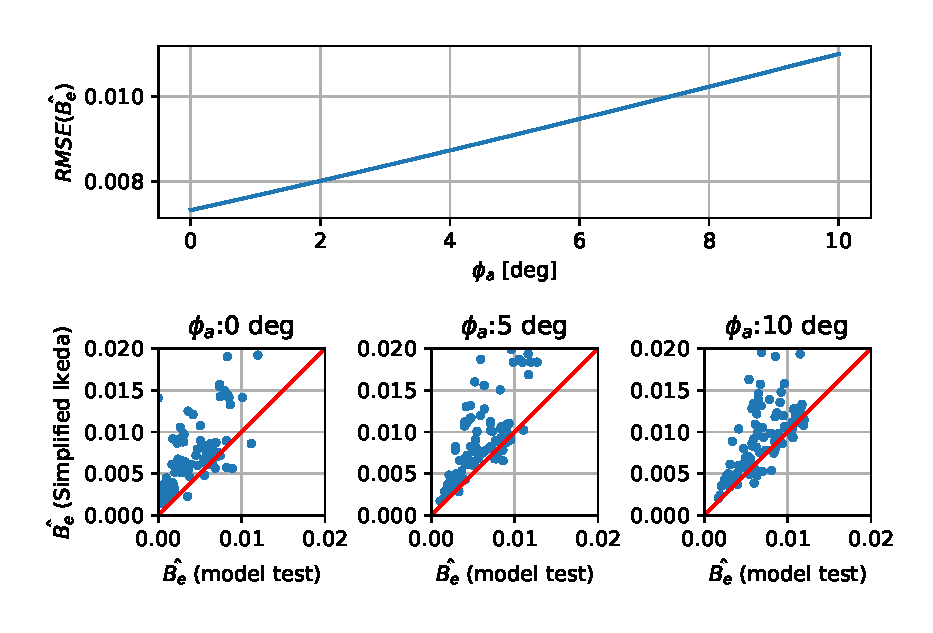
\includegraphics[]{figures/ikeda_phi_a.eps}
  \vspace{-0.5cm}
  \caption{Root mean square error of roll damping prediction between the SI-method and the model test results (upper plot). Influence of roll amplitude $\phi_a$ on $\hat{B_e}$ between the SI-method and model tests for $0^{\circ}$ (bottom left plot), $5^{\circ}$ (bottom middle plot) and $10^{\circ}$ (bottom right plot), respectively.}
  \label{fig:ikeda_phi_a}
\end{figure}

It was found that almost all ships in the roll damping database were outside the limits that are suitable to be applied in Eq.(\ref{eq:SI_limits}). Two different ways to handle this limit exceedance was investigated:
\begin{enumerate}
  \item the ``unlimited" approach where the input values are allowed to exceed the limits.
  \item the ``limited" approach where the limit boundary values were used for exceeding values.
\end{enumerate}

Fig.\ref{fig:ikeda_limited} show a comparison of predictions with ``unlimited" and ``limited" approach. The non-dimensional equivalent linear damping for roll amplitudes in the range 0 to 10 degrees are plotted against the corresponding results from model tests. The ``limited" approach seems to be the best one to use according to this figure, where the ``unlimited" approach has values very far away from the model test results (far away from the red reference line).   


\begin{figure}[H]
\vspace{-0.5cm}
\centering
  \centering
  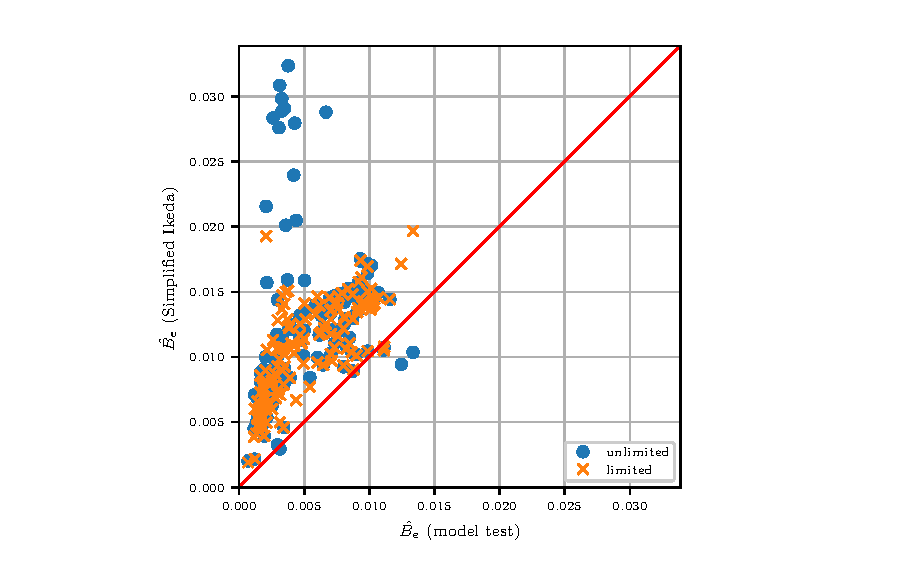
\includegraphics[]{figures/ikeda_limited.eps}
  \vspace{-0.5cm}
  \caption{$\hat{B_e}$ at all speeds estimated by the simplified Ikeda's method (Y-axis) in comparison with that from the roll decay test database (X-axis)}
  \label{fig:ikeda_limited}
\end{figure}
